\section{Introduction}
\subsection{The canonical example}
Let us consider the example from the abstract of water filtering through a porus medium, but this time in two dimensions. How do we model this? One might imagine that the medium consists of
many particles arranged (for simplicity) in an $n \times n$ square lattice and linked to each of their nearest neighbours. Clearly, this is the lattice on $\mathbb{Z}^2$.
To set up the problem, each of the particles will be expressed as a vertex in a graph and each of the links will be an edge. In the context of percolation, a vertex is called a site and an edge is
called a bond; these sites and bonds form a network.

\begin{definition}\label{def:site}
  A vertex in a graph is referred to as a \textbf{site}.
\end{definition}

\begin{definition}\label{def:bond}
  A edge in a graph is referred to as a \textbf{bond}.
\end{definition}

\begin{definition}\label{def:network}
  A graph is referred to as a \textbf{network}.
\end{definition}


So what does percolation actually mean? First we shall introduce the notion of open and closed sites and bonds and then we can discuss percolation.

\begin{definition}\label{def:open}
  A site or bond in a network is labeled \textbf{open} if it allows whatever we're considering to pass through.
\end{definition}

\begin{definition}\label{def:closed}
  A site or bond in a network is labeled \textbf{closed} if it doesn't allow whatever we're considering to pass through.
\end{definition}

And now for the percolation definitions.

\begin{definition}\label{def:site percolation}
  We say that we are considering \textbf{site percolation} if we let all of the sites in the network be open with probability $p \in [0, 1]$ and closed with probability $1-p \in
  [0, 1]$. We refer to $p$ here as the percolation probability.
\end{definition}
\begin{definition}\label{def:bond percolation}
  We say that we are considering \textbf{bond percolation} if we let all of the bonds in the network be open with probability $p \in [0, 1]$ and closed with probability $1-p \in
  [0, 1]$. We refer to $p$ here as the percolation probability.
\end{definition}

Now that we've defined site and bond percolation, what's the problem that we're trying to solve? In the case of water being poured on a porus medium, we would like to know
whether there is an open path from the top of the network to the bottom. We shall model this using site percolation (in fact, all examples in this essay will be using site
percolation unless explicitly stated otherwise).

\begin{definition}\label{def:open path}
  We say that a path in a network is \textbf{open} if:
  \begin{itemize}
    \item when considering site perolation, every site in the path is open.
    \item when considering bond percolation, every bond in the path is open.
  \end{itemize}
\end{definition}

\begin{definition}\label{def:openly connected}
  Let $N=(V, E)$ be a network and let $A, B \in V$. The sites $A, B$ are \textbf{openly connected} if there exists an open path connecting $A$ and $B$.
\end{definition}

\begin{definition}\label{def:openly disconnected}
  Let $N=(V, E)$ be a network and let $A, B \in V$. The sites $A, B$ are \textbf{openly disconnected} if there does not exist an open path connecting $A$ and
  $B$.\footnote{Definitions \ref{def:open path}, \ref{def:openly connected} and \ref{def:openly disconnected} are equivalent for both site and bond percolation.}
\end{definition}

The probability that an open path from the top of the network to the bottom exists depends on both our choices of both $p$ and $n$ from before. As a result of our context, our value for $n$ should be
large---this is the case with most percolation models---but we shall use small $n$ for the sake of example and simplicity. Let us now fix $n$ and see what happens as we vary $p$. Obviously we have two trivial cases, $p=0$ and $p=1$,
where the network is completely openly disconnected and completely openly connected respectively.
What about when $p\in(0,1)$? Let's inspect three different values of $p$ on our network: $p=0.25$, $p=0.5$ and $p=0.75$ as shown in figures \ref{fig:p=0.25}, \ref{fig:p=0.5} and
\ref{fig:p=0.75} on page \pageref{fig:probabilities}.
As one might expect, as $p$ increases, so does the "connectedness" of the network; i.e. the probability of having an open path from the top of the network to the bottom increases
with $p$. Also, observe that as $p$ increases we also get larger "clusters" of open connected sites or bonds.

\begin{definition}\label{def:cluster}
  Let $N=(V, E)$ be a network. A \textbf{cluster} is a set of vertices, $C \subset V$, such that if $v_1, v_2 \in C$ then $v_1$ and $v_2$ are openly connected.
\end{definition}

\begin{definition}\label{def:cluster size}
  Let $N=(V, E)$ be a network and let $C \subset V$ be a cluster. The \textbf{size} of $C$, denoted by $|C|$, is the number of sites in the cluster. A cluster of size $s$ may be
  referred to as an $s$-cluster.
\end{definition}

\begin{figure}[p]
  \centering
  \begin{subfigure}[b]{0.45\textwidth}
    \centering
    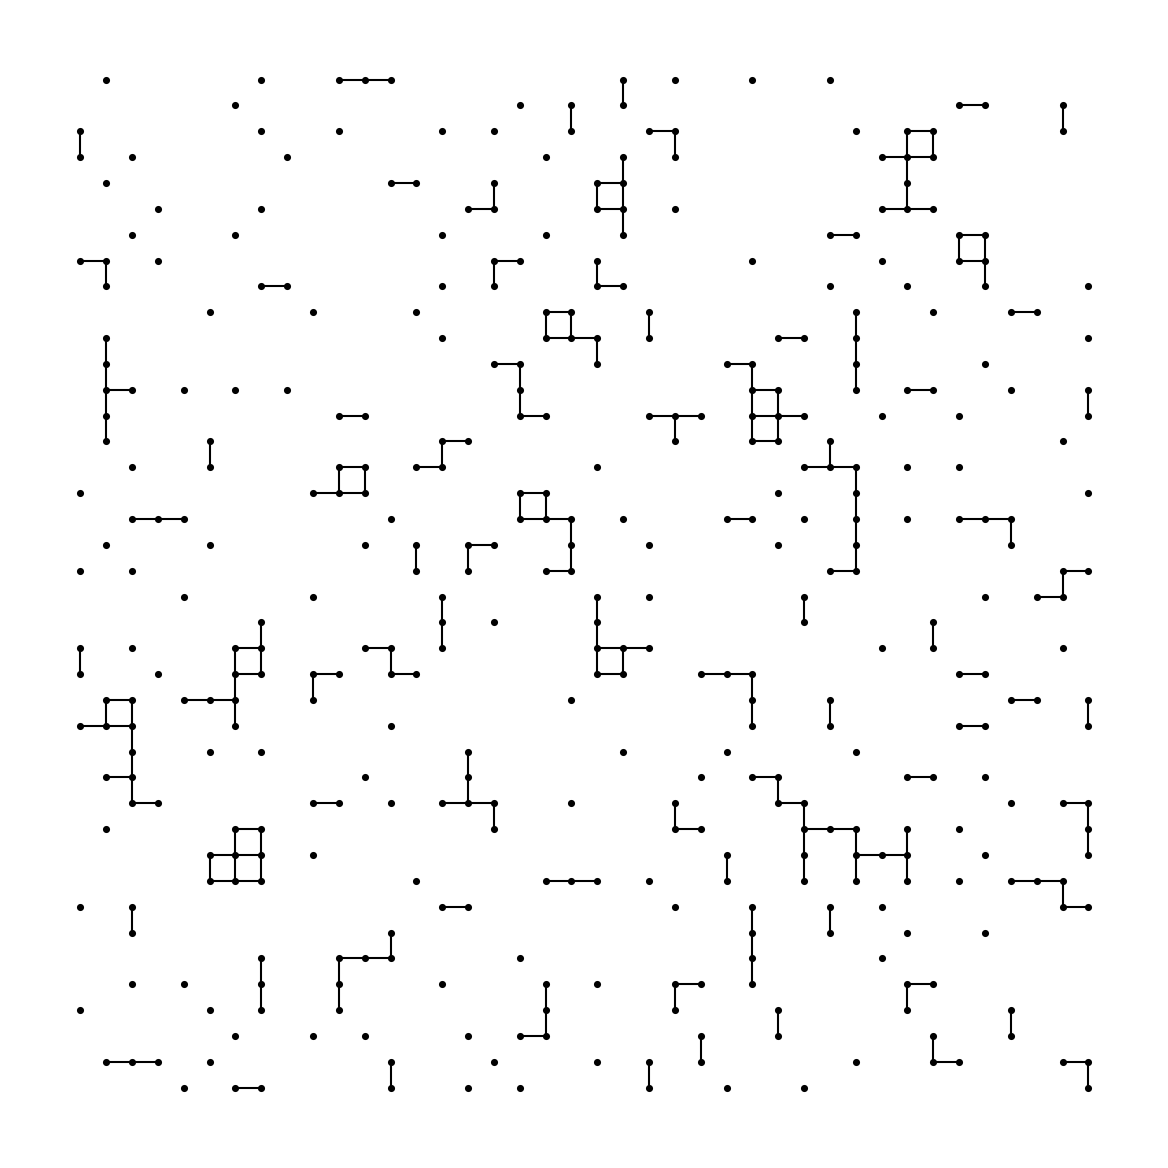
\includegraphics[width=\textwidth]{1/percolation1}
    \caption{$p=0.25$}
    \label{fig:p=0.25}
  \end{subfigure}
  \hfill
  \begin{subfigure}[b]{0.45\textwidth}
    \centering
    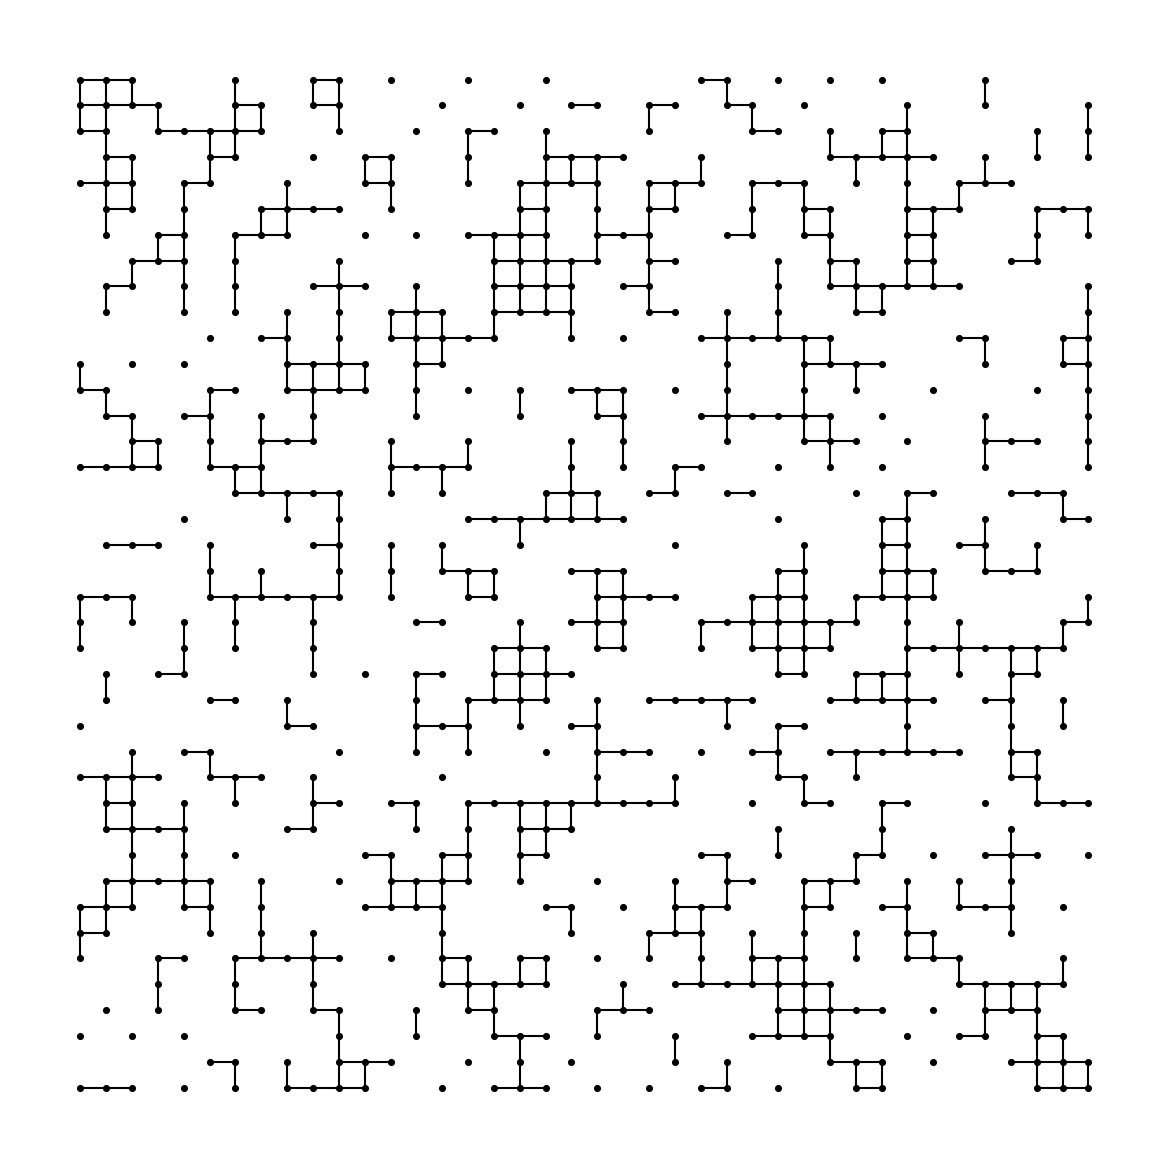
\includegraphics[width=\textwidth]{1/percolation2}
    \caption{$p=0.5$}
    \label{fig:p=0.5}
  \end{subfigure}
  \hfill
  \begin{subfigure}[b]{0.45\textwidth}
    \centering
    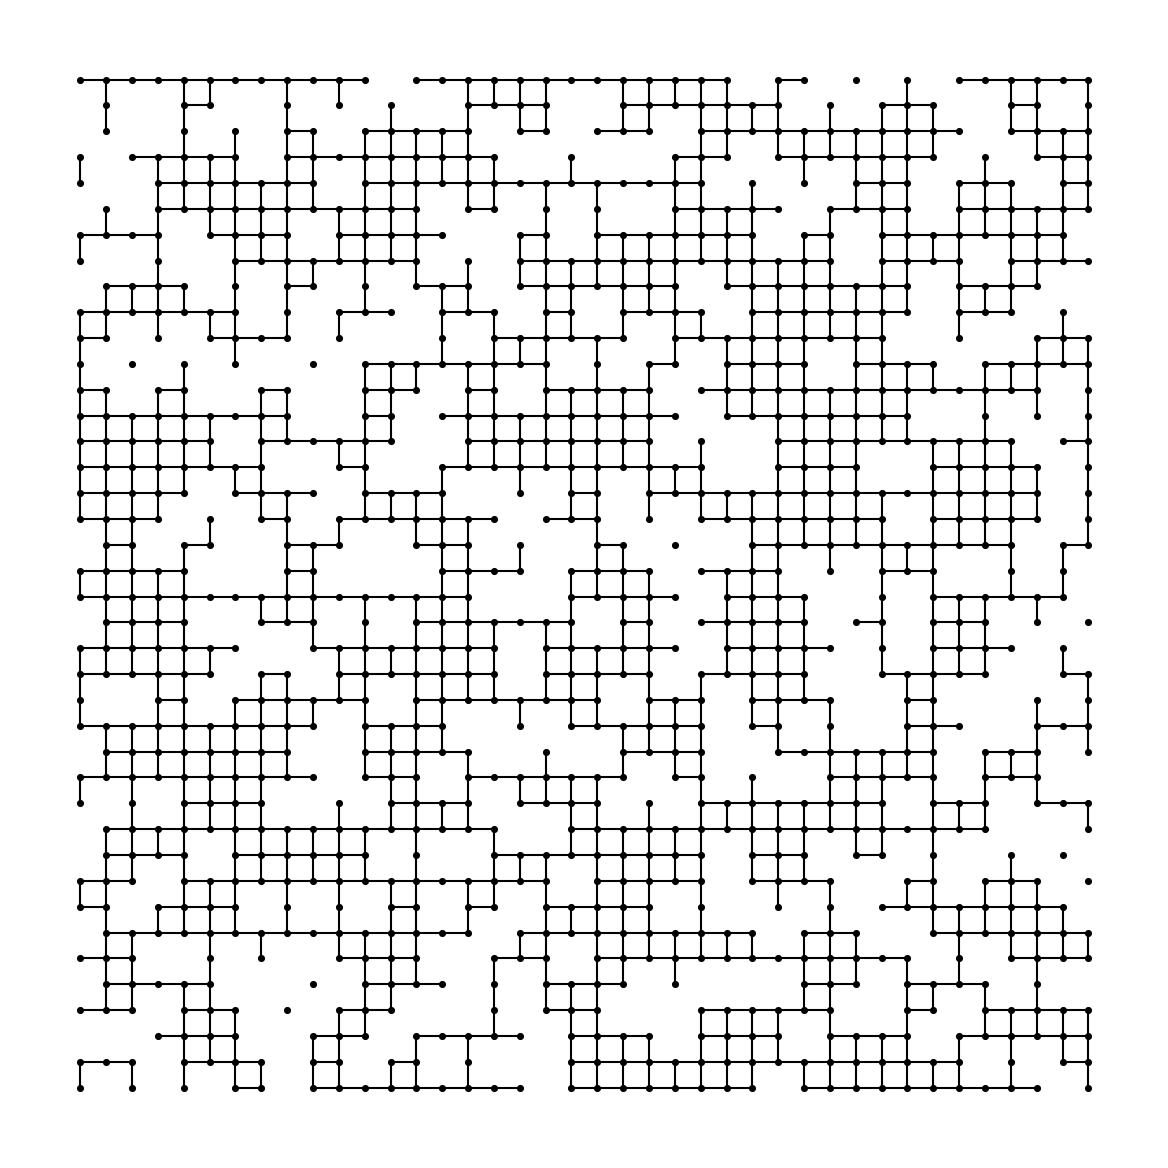
\includegraphics[width=\textwidth]{1/percolation3}
    \caption{$p=0.75$}
    \label{fig:p=0.75}
  \end{subfigure}
  \caption{Examples of \textit{bond} percolation for $p\in(0,1)$ on a $40 \times 40$ network.}
  \label{fig:probabilities}
\end{figure}

We will explore clusters in more detail in the next section, but for now let us introduce the idea of a critical probability. Although they don't exist in the finite cases, they do
exist in the infinite cases. 

\begin{definition}\label{def:infinite cluster}
  Consider a network, $N = (V, E)$. A cluster, $C \subseteq V$, is considered \textbf{infinite} if and only if $|C| = \infty$.
\end{definition}

\begin{definition}\label{def:critical probability}
  Consider an infinite network $N = (V, E)$. The \textbf{critical probability}, denoted $p_c$, is the percolation probabililty such that the probability that there exists a
  cluster, $C \subseteq V$ with $|C| = \infty$ is $1$.
  \todo{Add computational examples of the connectedness as p changes}
\end{definition}
% \newpage

\subsection{Other network configurations}
We have already seen the lattice on $\mathbb{Z}^2$ as an example, but there are many more. To remain within the scope of this essay, we shall only breifly mention some two and
three dimensional examples and print their site and bond critical probabilities and a diagram.

\begin{definition}
  A network is considered \textbf{regular} if every site in that network has the same number of bonds attached to it.
\end{definition}

\begin{definition}
  The \textbf{coordination number} of a regular network is the number of bonds attached at every site. This quantity is denoted using the letter $Z$. I.e. the lattice on
  $\mathbb{Z}^2$ has a coordination number $Z = 4$. 
\end{definition}

\subsection*{Two dimensional network configurations}
Clearly, one two dimensional network configuration is the lattice on $\mathbb{Z}^2$. In context this is referred to as the square lattice. Other regular two dimensional network configurations include, but are not limited to, the Bethe Lattice (Figure \ref{fig:bethe lattice}), Honeycomb
Lattice (Figure \ref{fig:honeycomb lattice}), Kagome Lattice (Figure \ref{fig:kagome lattice}) and the Triangular Lattice (Figure \ref{fig:triangular lattice}). As one might
imagine, each of these configurations has a different (but not necessarily distinct) critical probability. Below is a table showing the critical probabilities for each of the
aforementioned network configurations. It should be noted that probabilities marked with a * (star) are exact results. \cite[p. 11]{Sahimi}

\begin{figure}[h!]
\begin{center}
\begin{tabular}{| c | c | c | c |}
    \hline
    Configuration & Z & $p_c$ for bond percolation & $p_c$ for site percolation \\
    \hline
    Bethe & $3$ & TO FIND & TO FIND \\
    Honeycomb & $3$ & $1 - 2\sin(\pi/18)$* & $0.6962$ \\
    $\mathbb{Z}^2$ (Square) & $4$ & $1/2$* & $0.5927$ \\
    Kagome & $4$ & $0.522$ & $0.652$ \\
    Triangular & $6$ & $2\sin(\pi/18)$* & $1/2$* \\
    \hline
  \end{tabular}
\end{center}
\centering
\caption{Critical probabilities for various configurations of two dimensional networks}
\label{fig:critical probabilities in two dimensions}
\end{figure}

\begin{figure}[h!]
\begin{center}
\begin{tabular}{| c | c | c | c |}
    \hline
    Configuration & Z & $p_c$ for site percolation & $p_c$ for bond percolation \\
    \hline
    Diamond & $4$ & $0.3886$ & $0.4299$ \\
    Simple Cubic & $6$ & $0.2488$ & $0.3116$ \\
    BCC & $8$ & $0.1795$ & $0.2464$ \\
    FCC & $12$ & $0.198$ & $0.119$ \\
    \hline
  \end{tabular}
\end{center}
\centering
\caption{Critical probabilities for various configurations of three dimensional networks}
\label{fig:critical probabilities in three dimensions}
\end{figure}

\begin{figure}[p]
  \centering
  \begin{subfigure}[b]{0.45\textwidth}
    \centering
    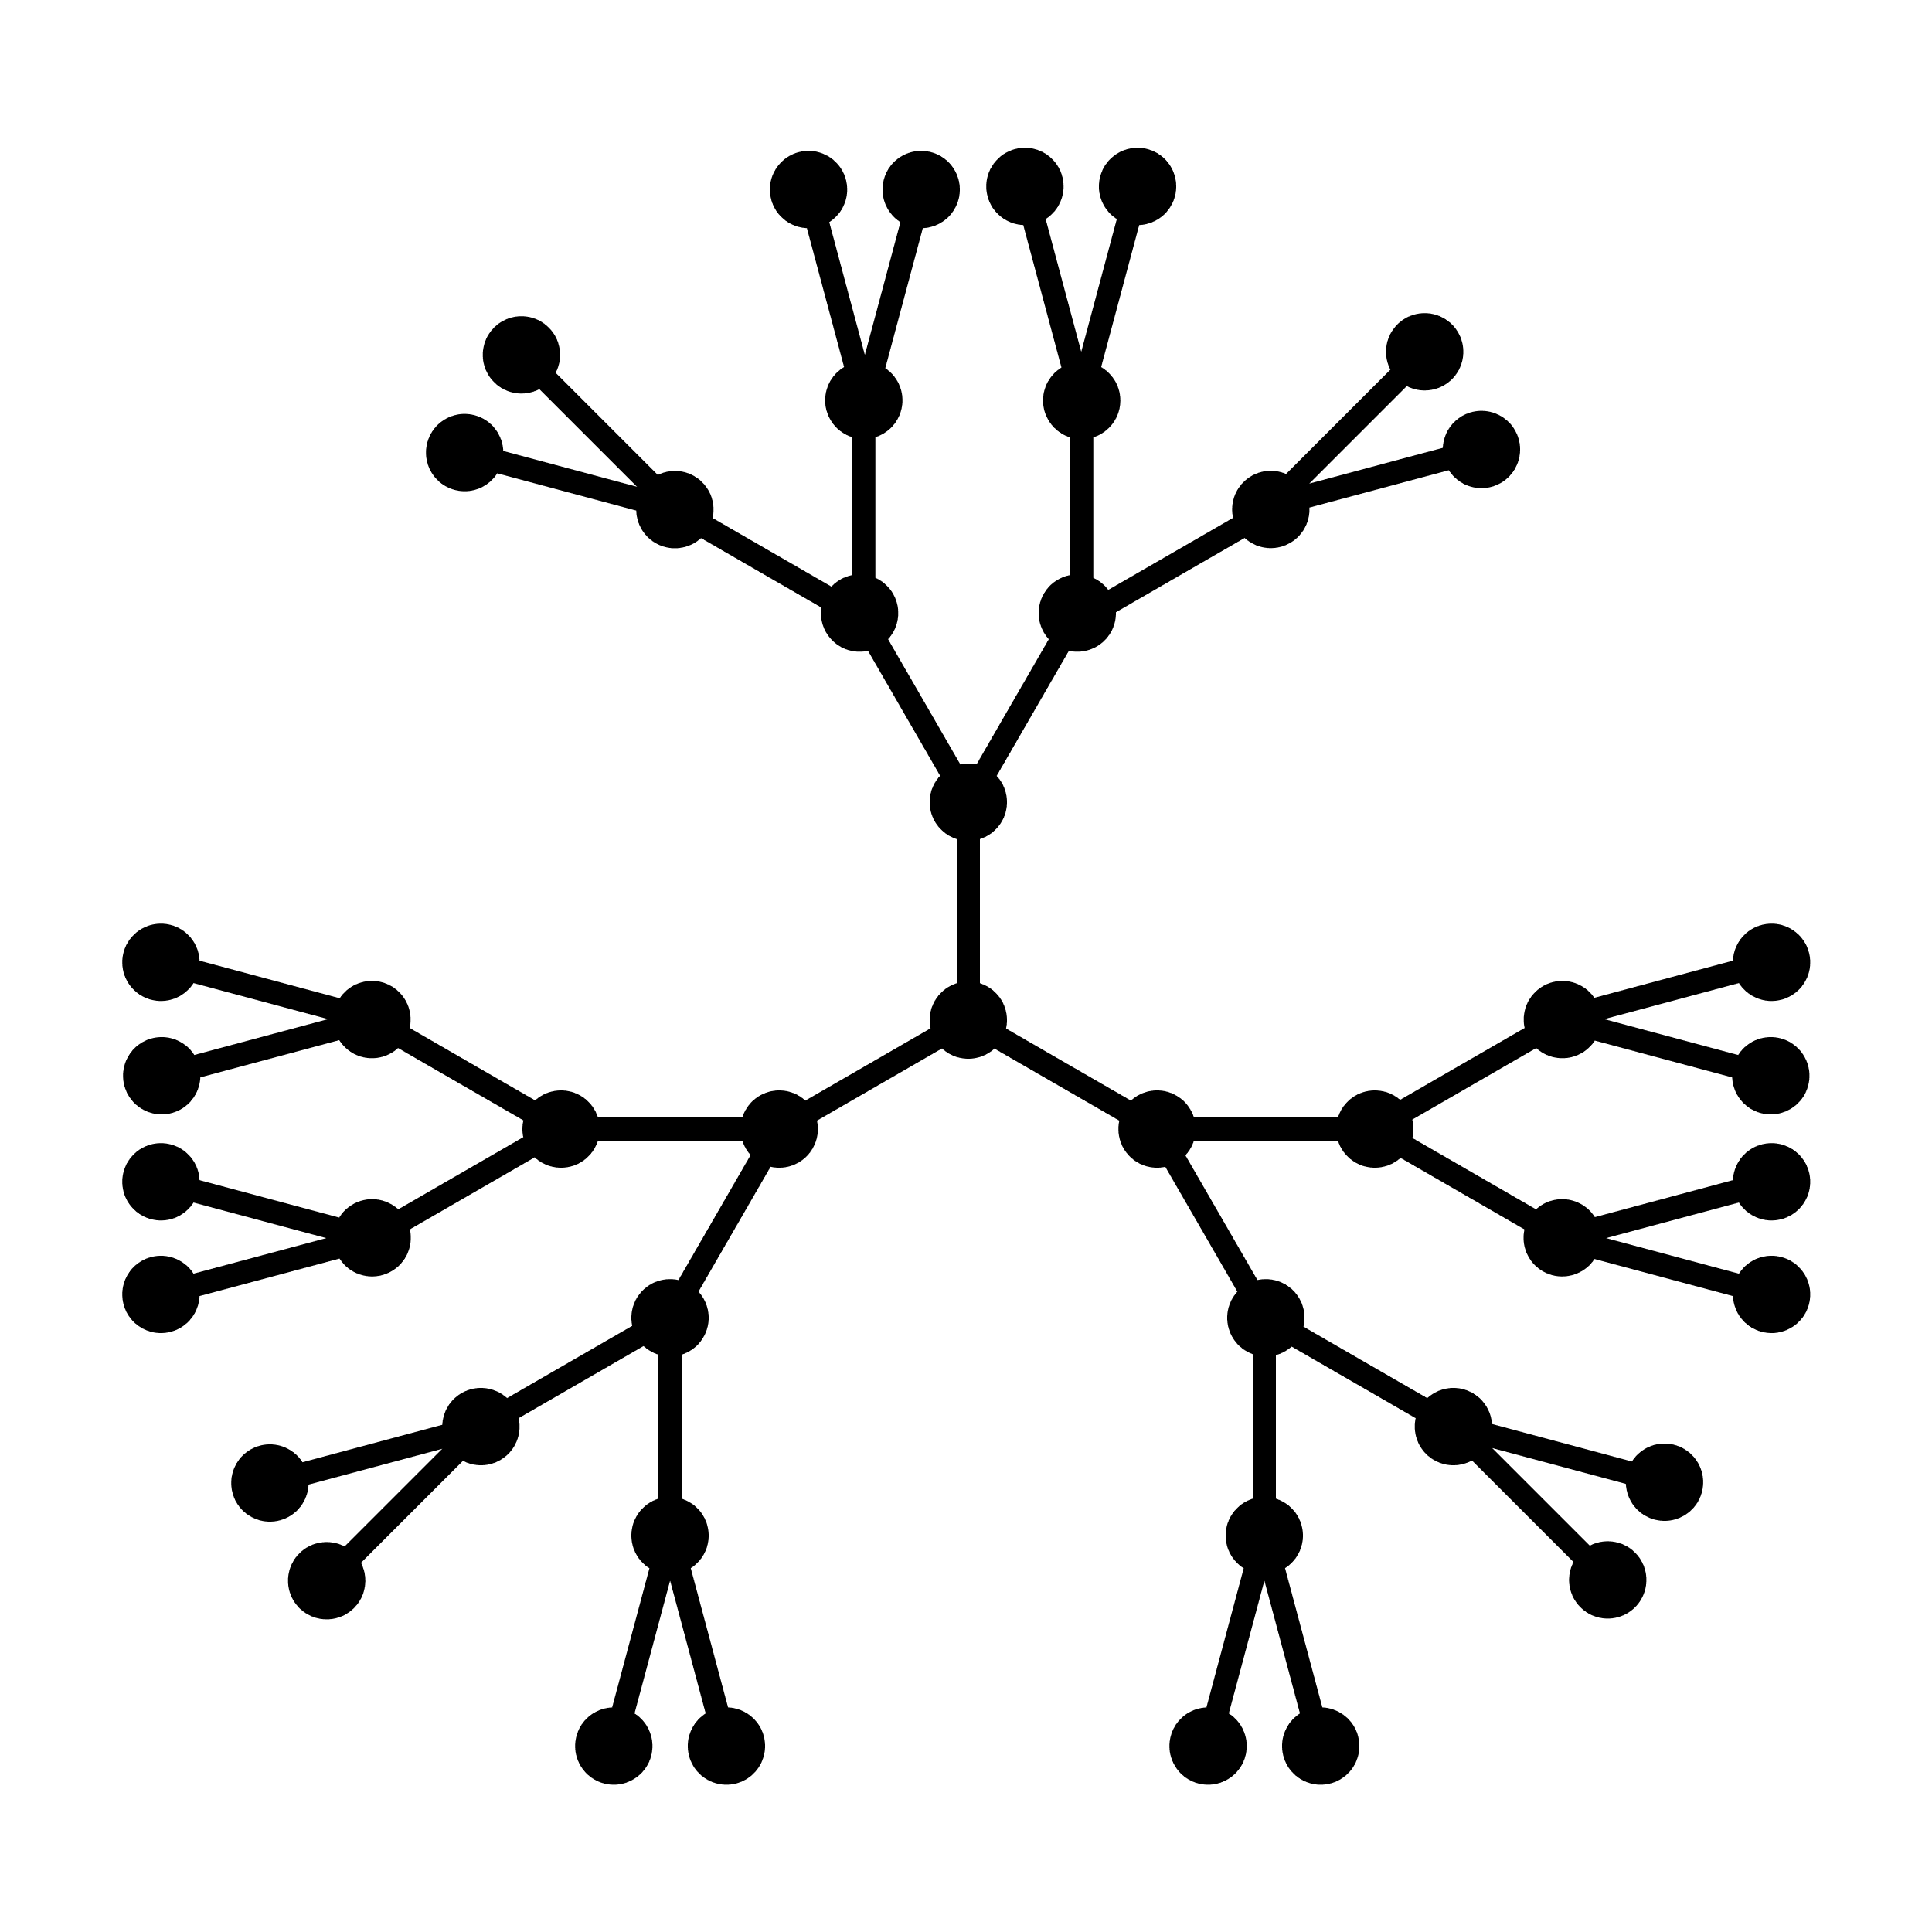
\includegraphics[width=\textwidth]{2/Bethe}
    \caption{Bethe Lattice}
    \label{fig:bethe lattice}
  \end{subfigure}
  \hfill
  \begin{subfigure}[b]{0.45\textwidth}
    \centering
    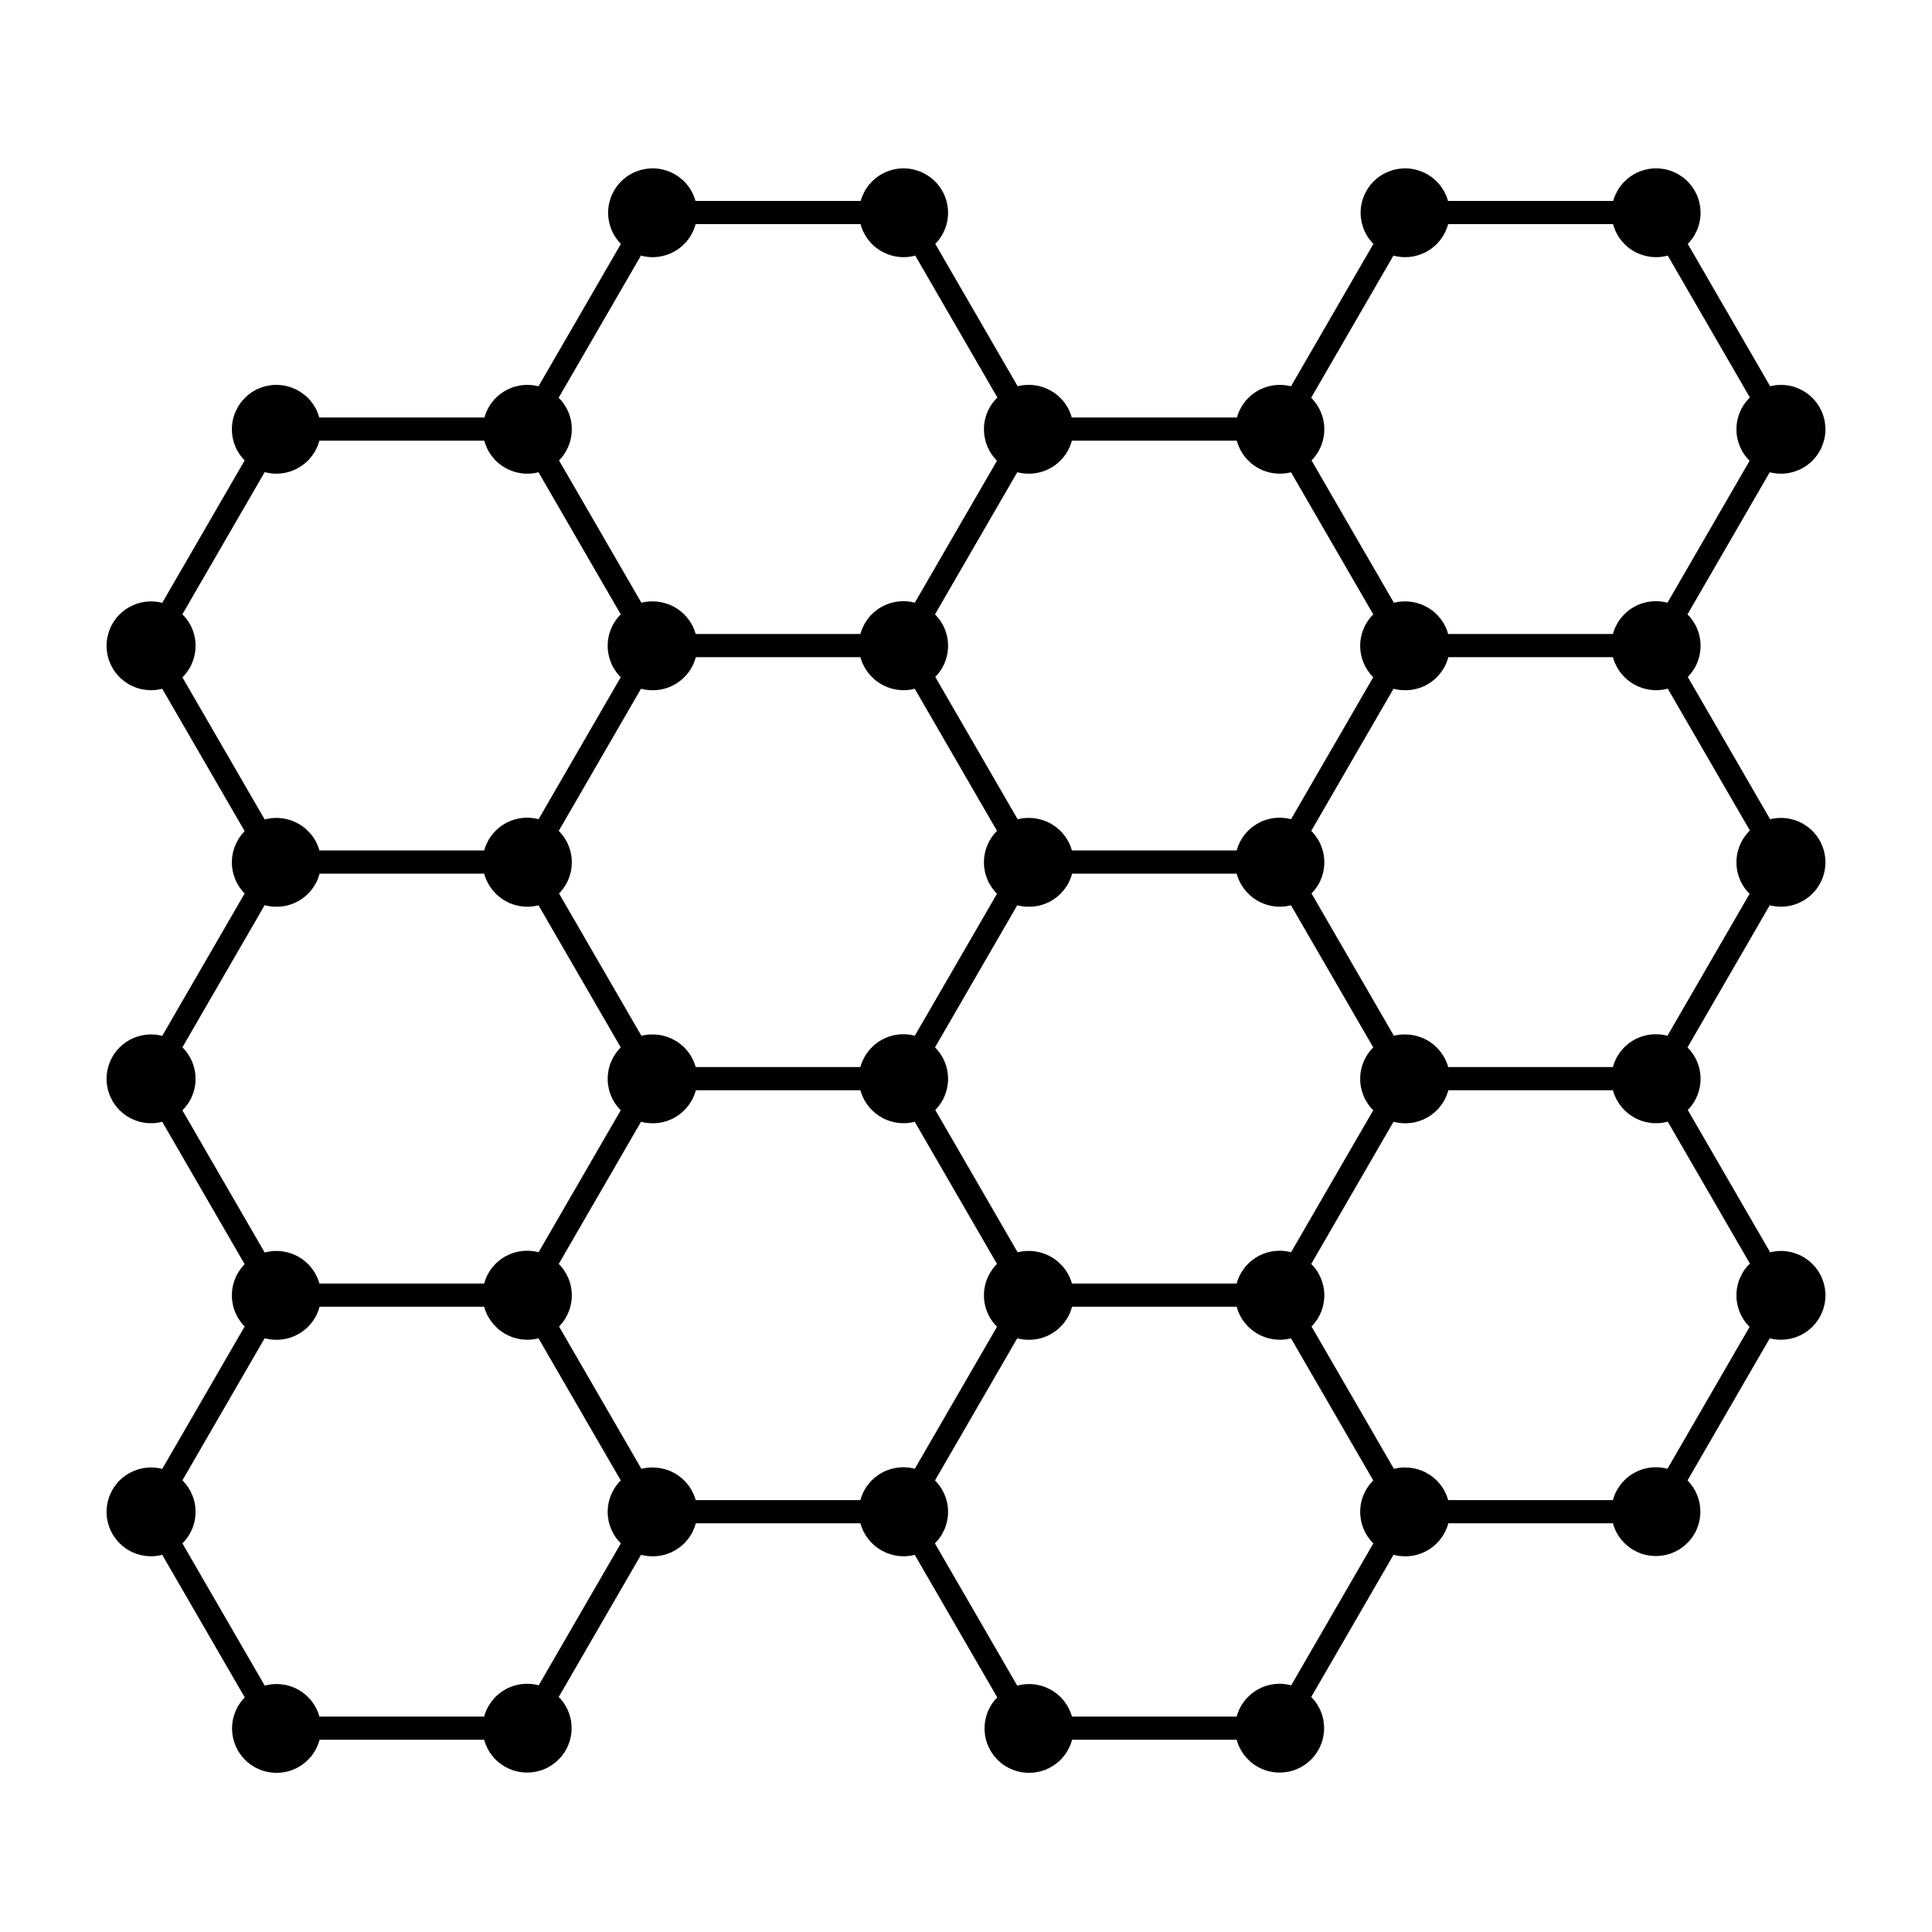
\includegraphics[width=\textwidth]{2/Honeycomb}
    \caption{Honeycomb Lattice}
    \label{fig:honeycomb lattice}
  \end{subfigure}
  \hfill
  \begin{subfigure}[b]{0.45\textwidth}
    \centering
    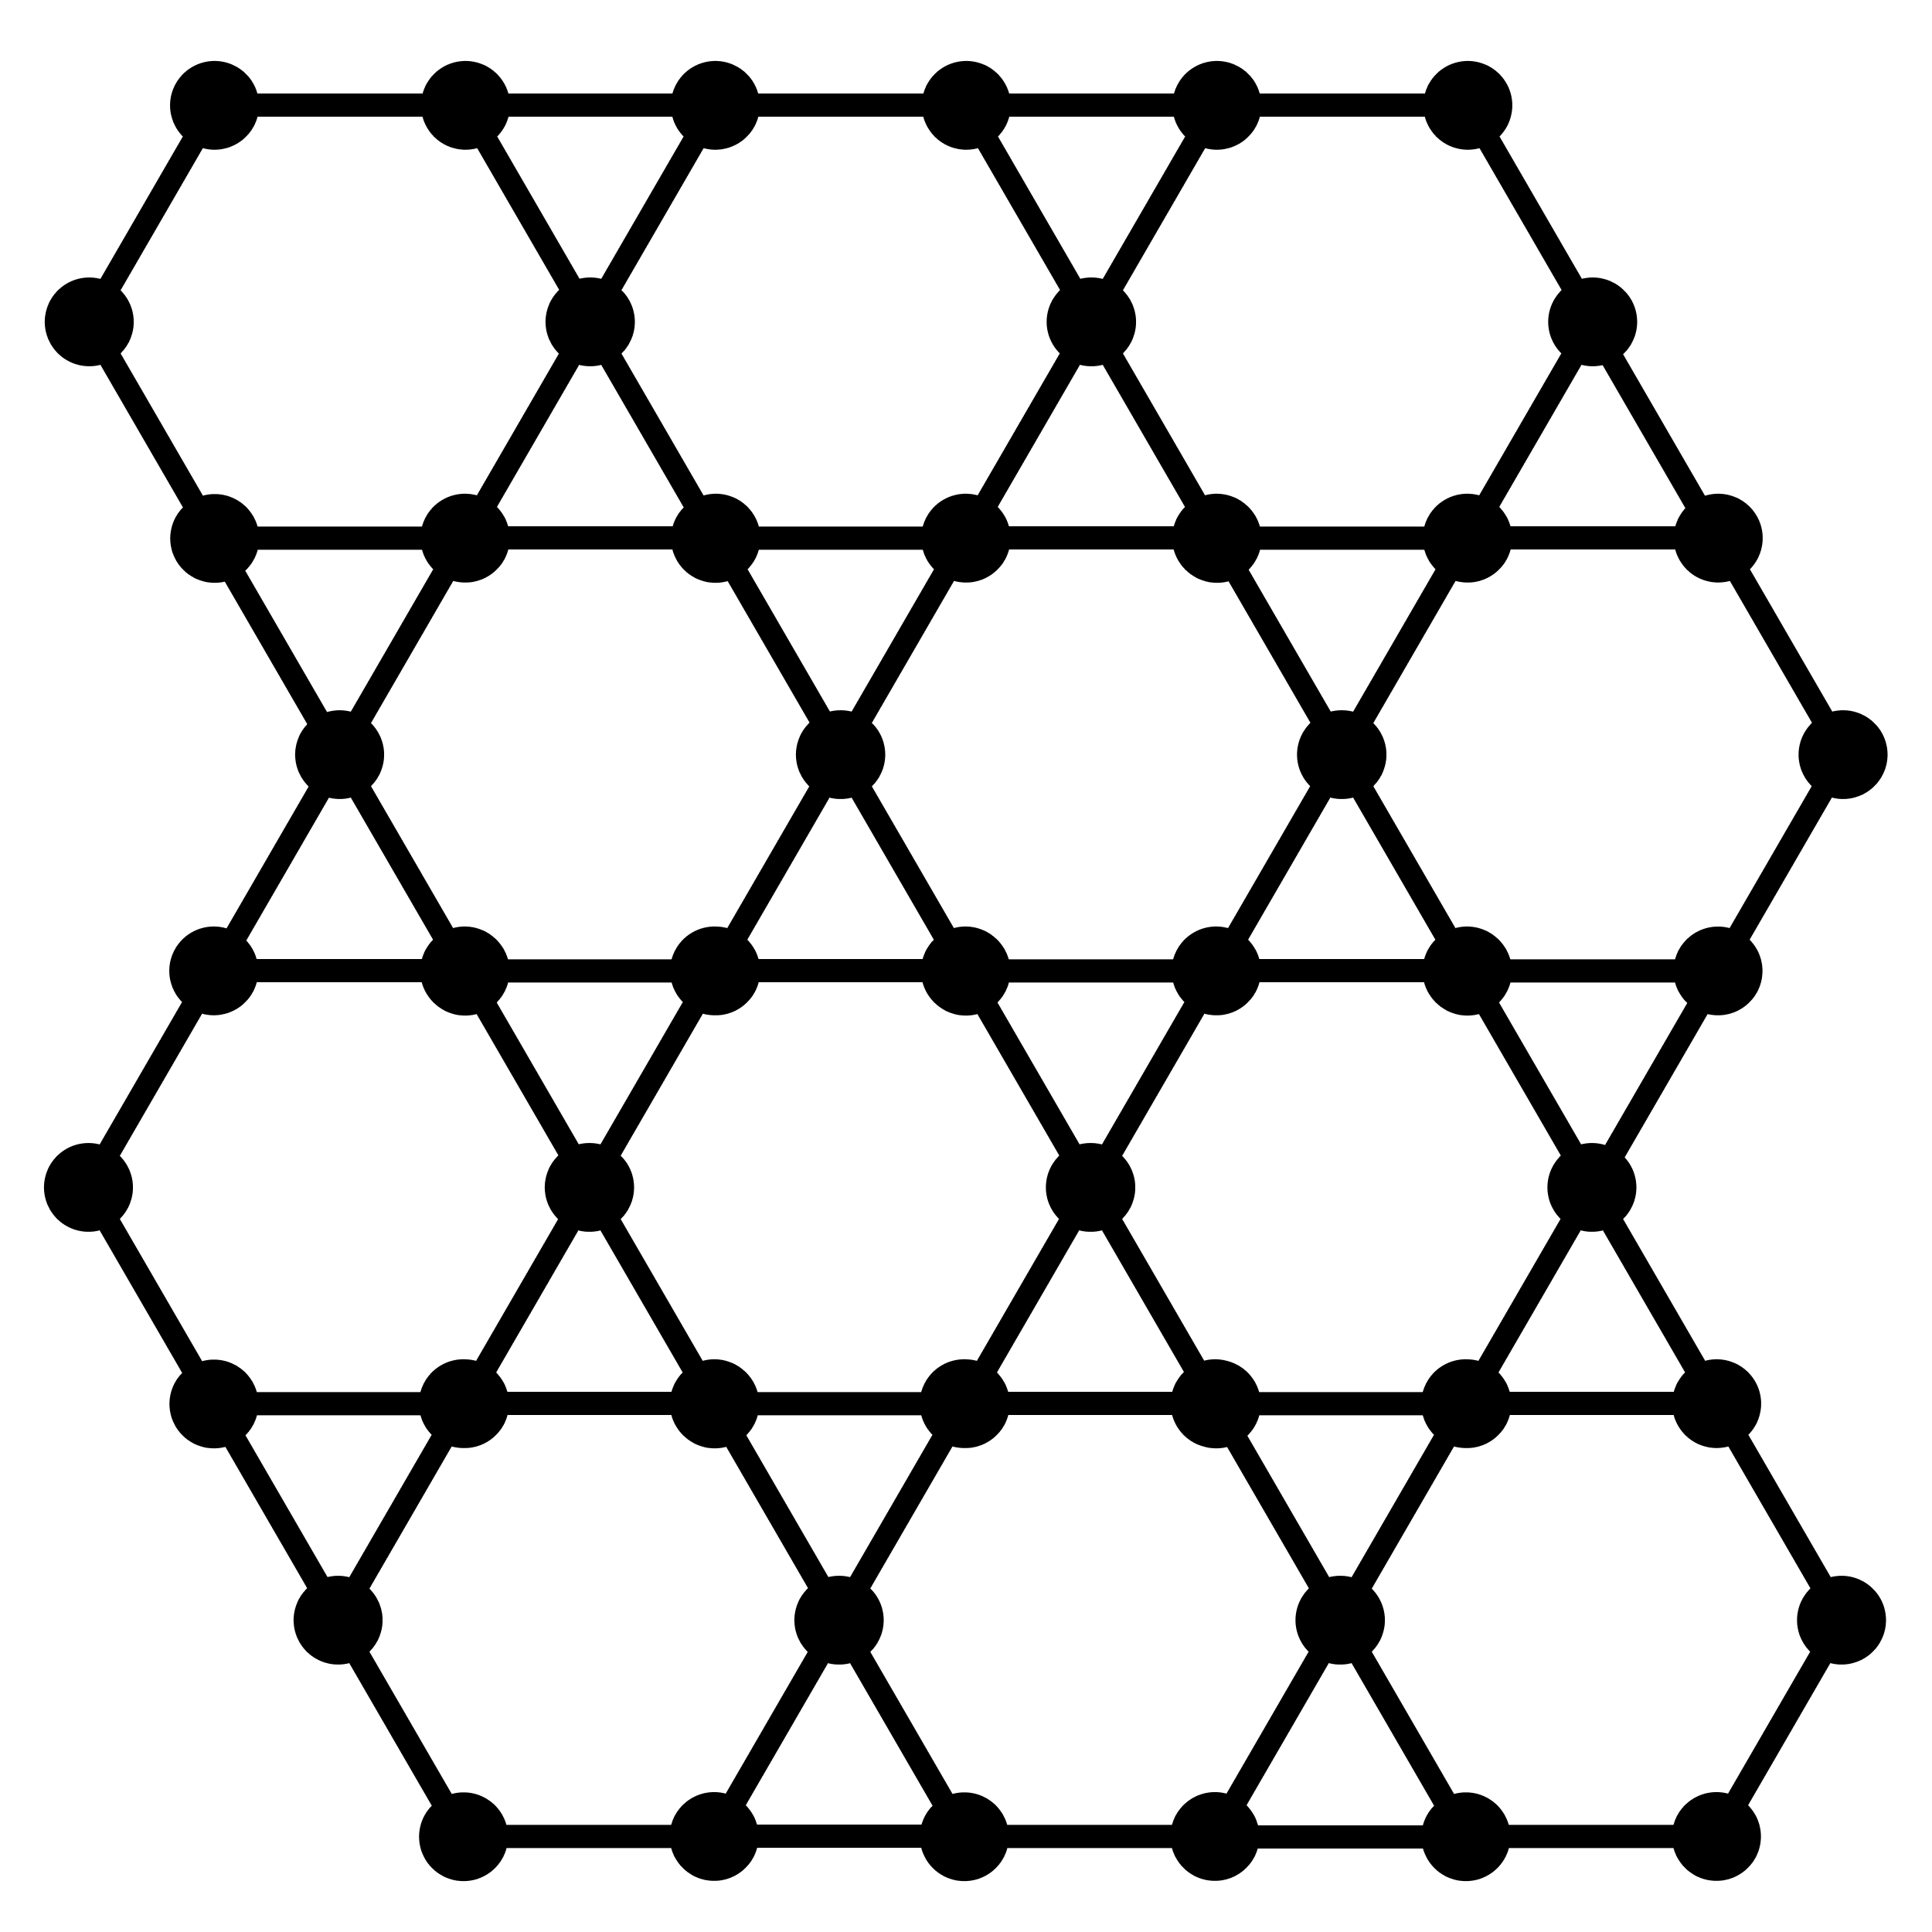
\includegraphics[width=\textwidth]{2/Kagome}
    \caption{Kagome Lattice}
    \label{fig:kagome lattice}
  \end{subfigure}
  \hfill
  \begin{subfigure}[b]{0.45\textwidth}
    \centering
    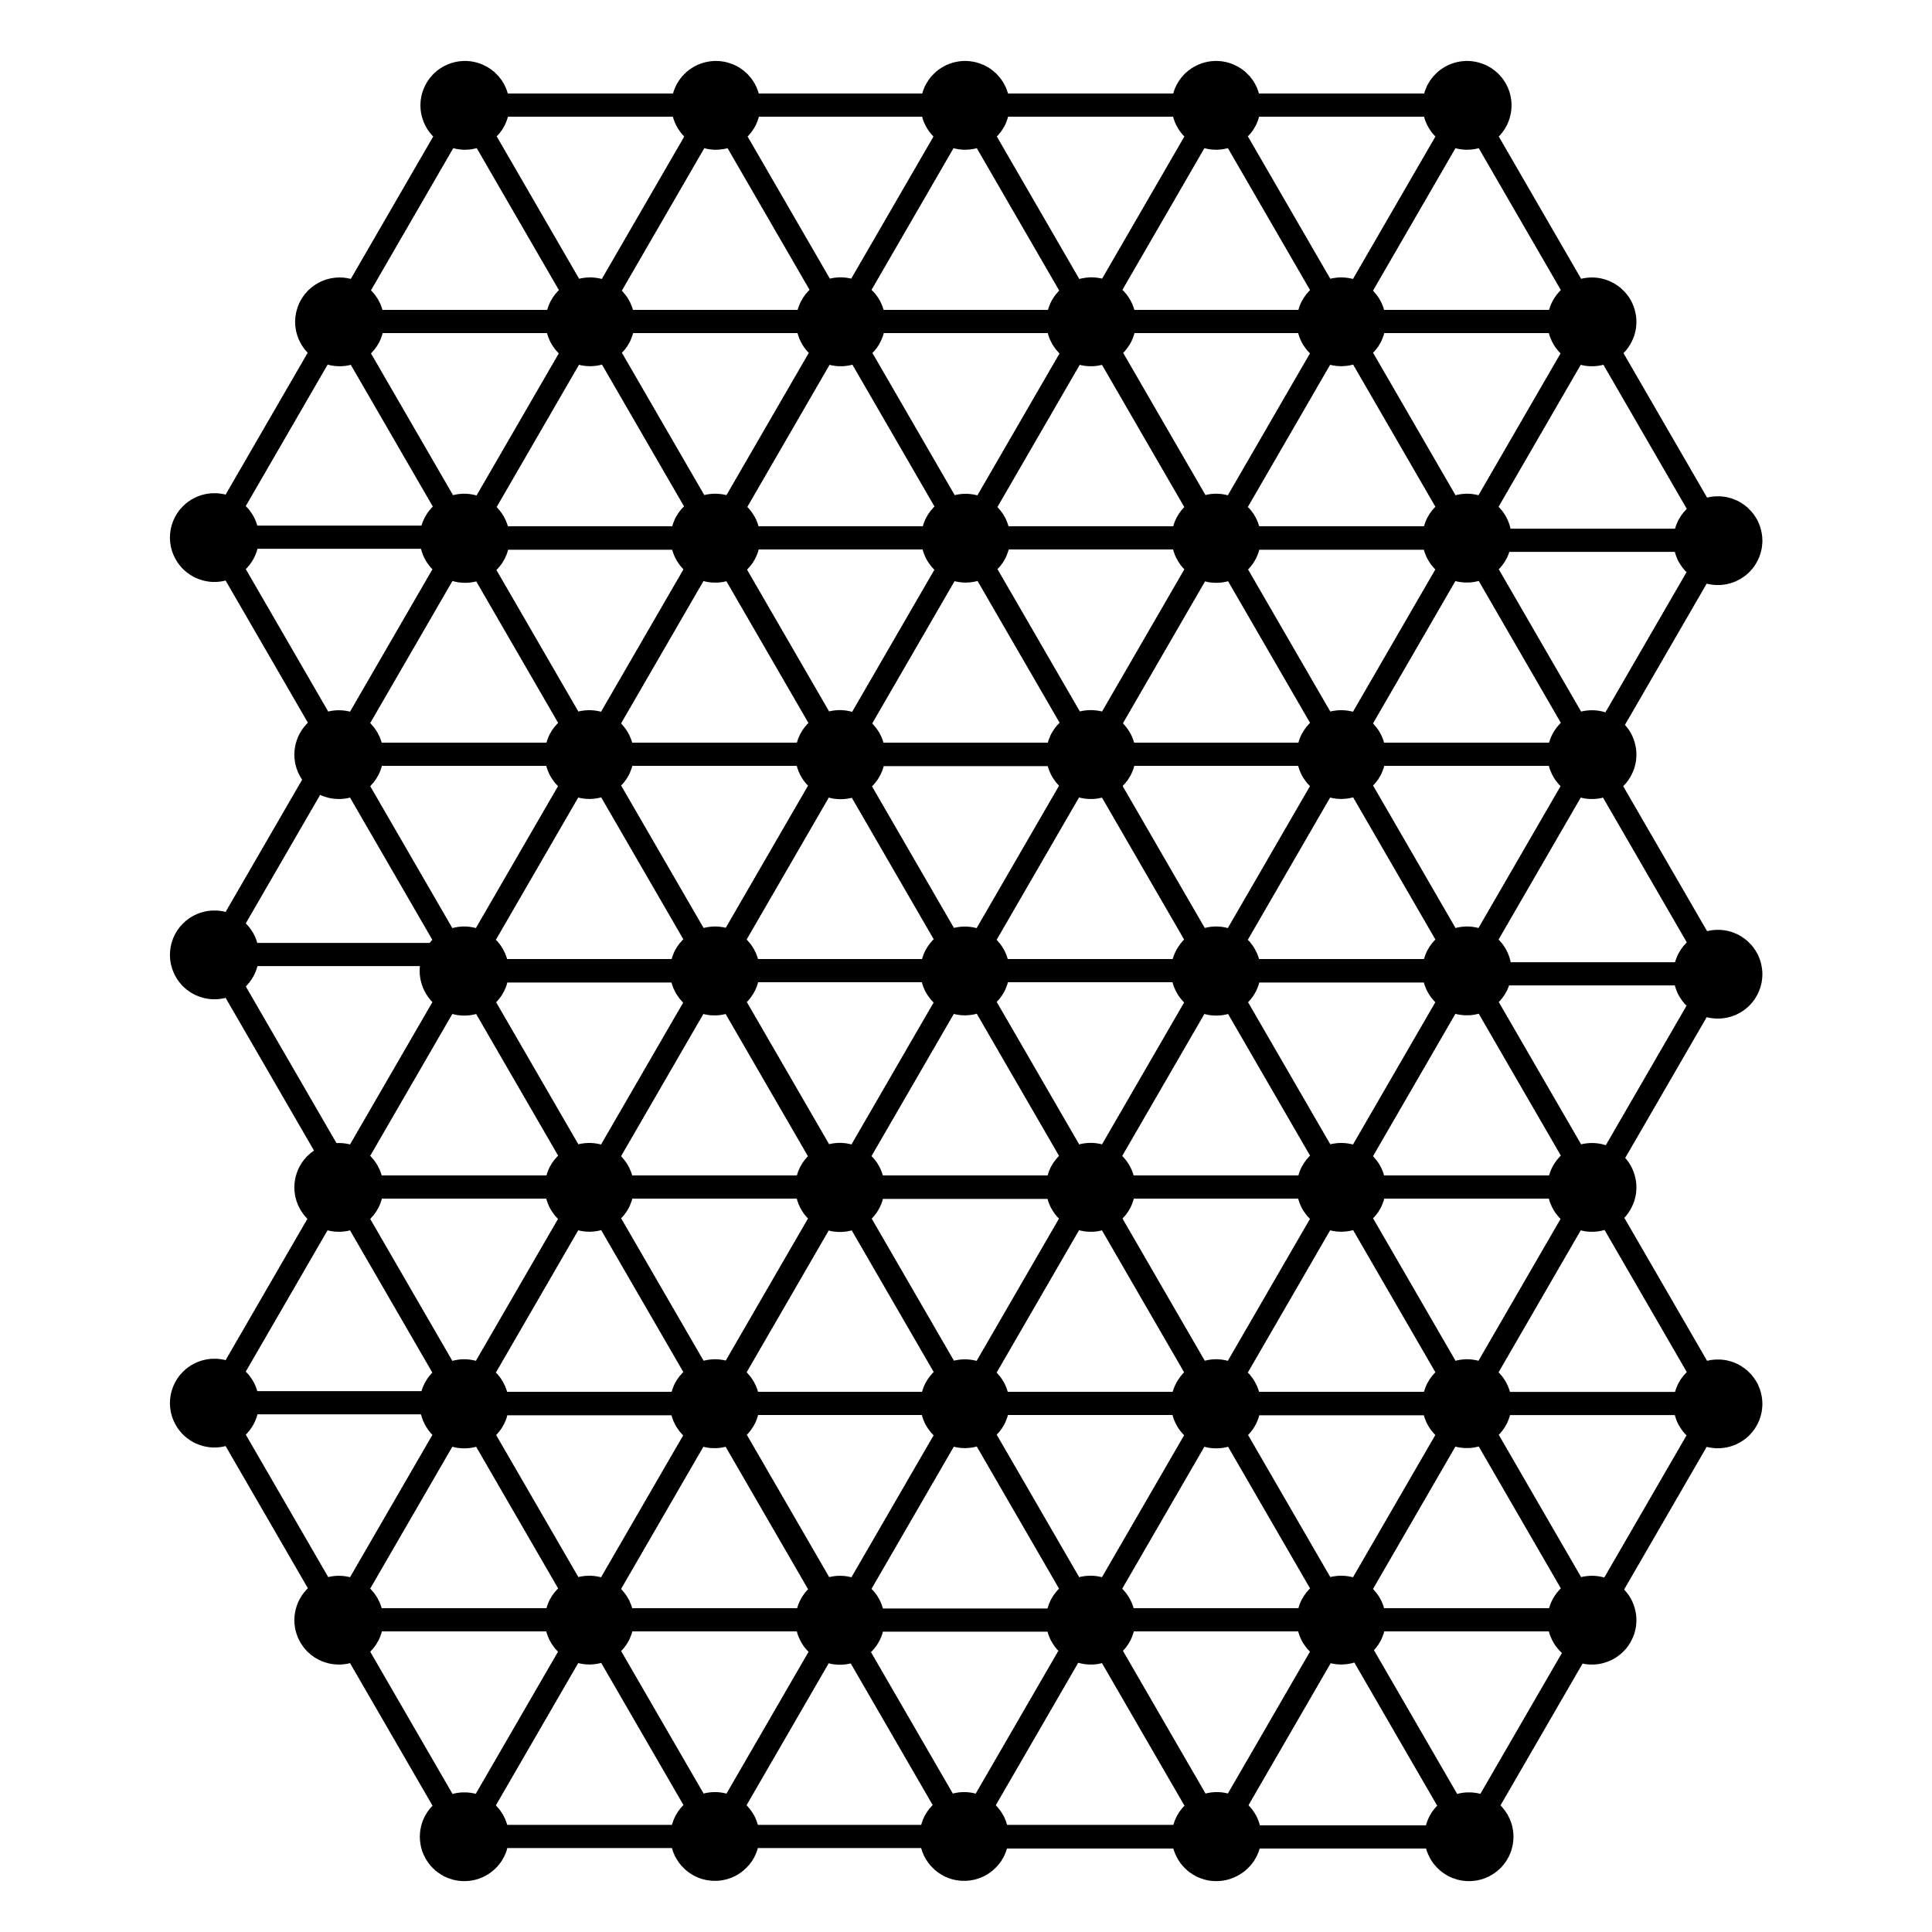
\includegraphics[width=\textwidth]{2/Triangular}
    \caption{Triangular Lattice}
    \label{fig:triangular lattice}
  \end{subfigure}
  \caption{Two dimensional regular network configurations}
  \label{fig:two dimensional networks}
\end{figure}

\subsection*{Three dimensional network configurations}
It shouldn't be hard to guess that the lattice on $\mathbb{Z}^3$ is a potential configuration for three dimensional networks. We call this configuration the Simple Cubic Lattice (Figure
\ref{fig:simple cubic lattice}). Similarly to
the two dimensional case, there many other regular three dimensional network configurations. These include, but again are not limited to, the Diamond Lattice (Figure
\ref{fig:diamond lattice}), the Body Centered Cubic (BCC) Lattice (Figure \ref{fig:body centered cubic lattice}) and the Face Centered Cubic (FCC) Lattice (Figure \ref{fig:face
centered cubic lattice}). Notice how none of these results are precise. \cite[p. 11]{Sahimi}

\begin{figure}[p]
  \centering
  \begin{subfigure}[b]{0.45\textwidth}
    \centering
    
\includegraphics[width=\textwidth]{images/placeholder}
    \caption{Diamond Lattice}
    \label{fig:diamond lattice}
  \end{subfigure}
  \hfill
  \begin{subfigure}[b]{0.45\textwidth}
    \centering
    
\includegraphics[width=\textwidth]{images/placeholder}
    \caption{Simple Cubic Lattice}
    \label{fig:simple cubic lattice}
  \end{subfigure}
  \hfill
  \begin{subfigure}[b]{0.45\textwidth}
    \centering
    
\includegraphics[width=\textwidth]{images/placeholder}
    \caption{Body Centered Cubic Lattice}
    \label{fig:body centered cubic lattice}
  \end{subfigure}
  \hfill
  \begin{subfigure}[b]{0.45\textwidth}
    \centering
    
\includegraphics[width=\textwidth]{images/placeholder}
    \caption{Face Centered Cubic Lattice}
    \label{fig:face centered cubic lattice}
  \end{subfigure}
  \caption{Three dimensional regular network configurations}
  \label{fig:three dimensional networks}
\end{figure}
